\section{System Demonstration}
\par The demonstration consists of three parts. (1) we demonstrate its ranking models and heterogenous entity rankings given the query keywords by \oursystem. (2) To further illustrate the effective ranking model based on importance, we take {\em time ranking} in SIGMOD as an example. (3) We also demonstrate author profiling for a better knowledge of the author.


\stitle{Article Ranking and Keywords Profiling}. Fig. \ref{fig: search keywords} is an example of Search Page. In this page, we fulfill the query need with their ranking metrics and construct keywords profiling,
try to answer which authors/venues/affiliations are the most authoritative in the queried field of study.

\par

It has four major areas: (1) Area 1, the top of the picture, where users can search keywords, authors, affiliations, journal and conference (2) Area 2 presents influential papers about the keywords and {\em relevance} for default ranking metric, which is in the center of the picture. (3) At left of the picture is Area 3, users can specify different ranking metrics such as {\em relevance}, {\em importance}, {\em citation}, {\em year} to fit various ranking scenarios. (4) Top-k prestige authors, influential affiliations, famous journals/conferences corresponding to ranking metrics and keywords are shown in Area 4, which is at the right of the picture.

% keywords search and profiling.

\stitle{Ranking Instance}


\begin{figure}
\centering
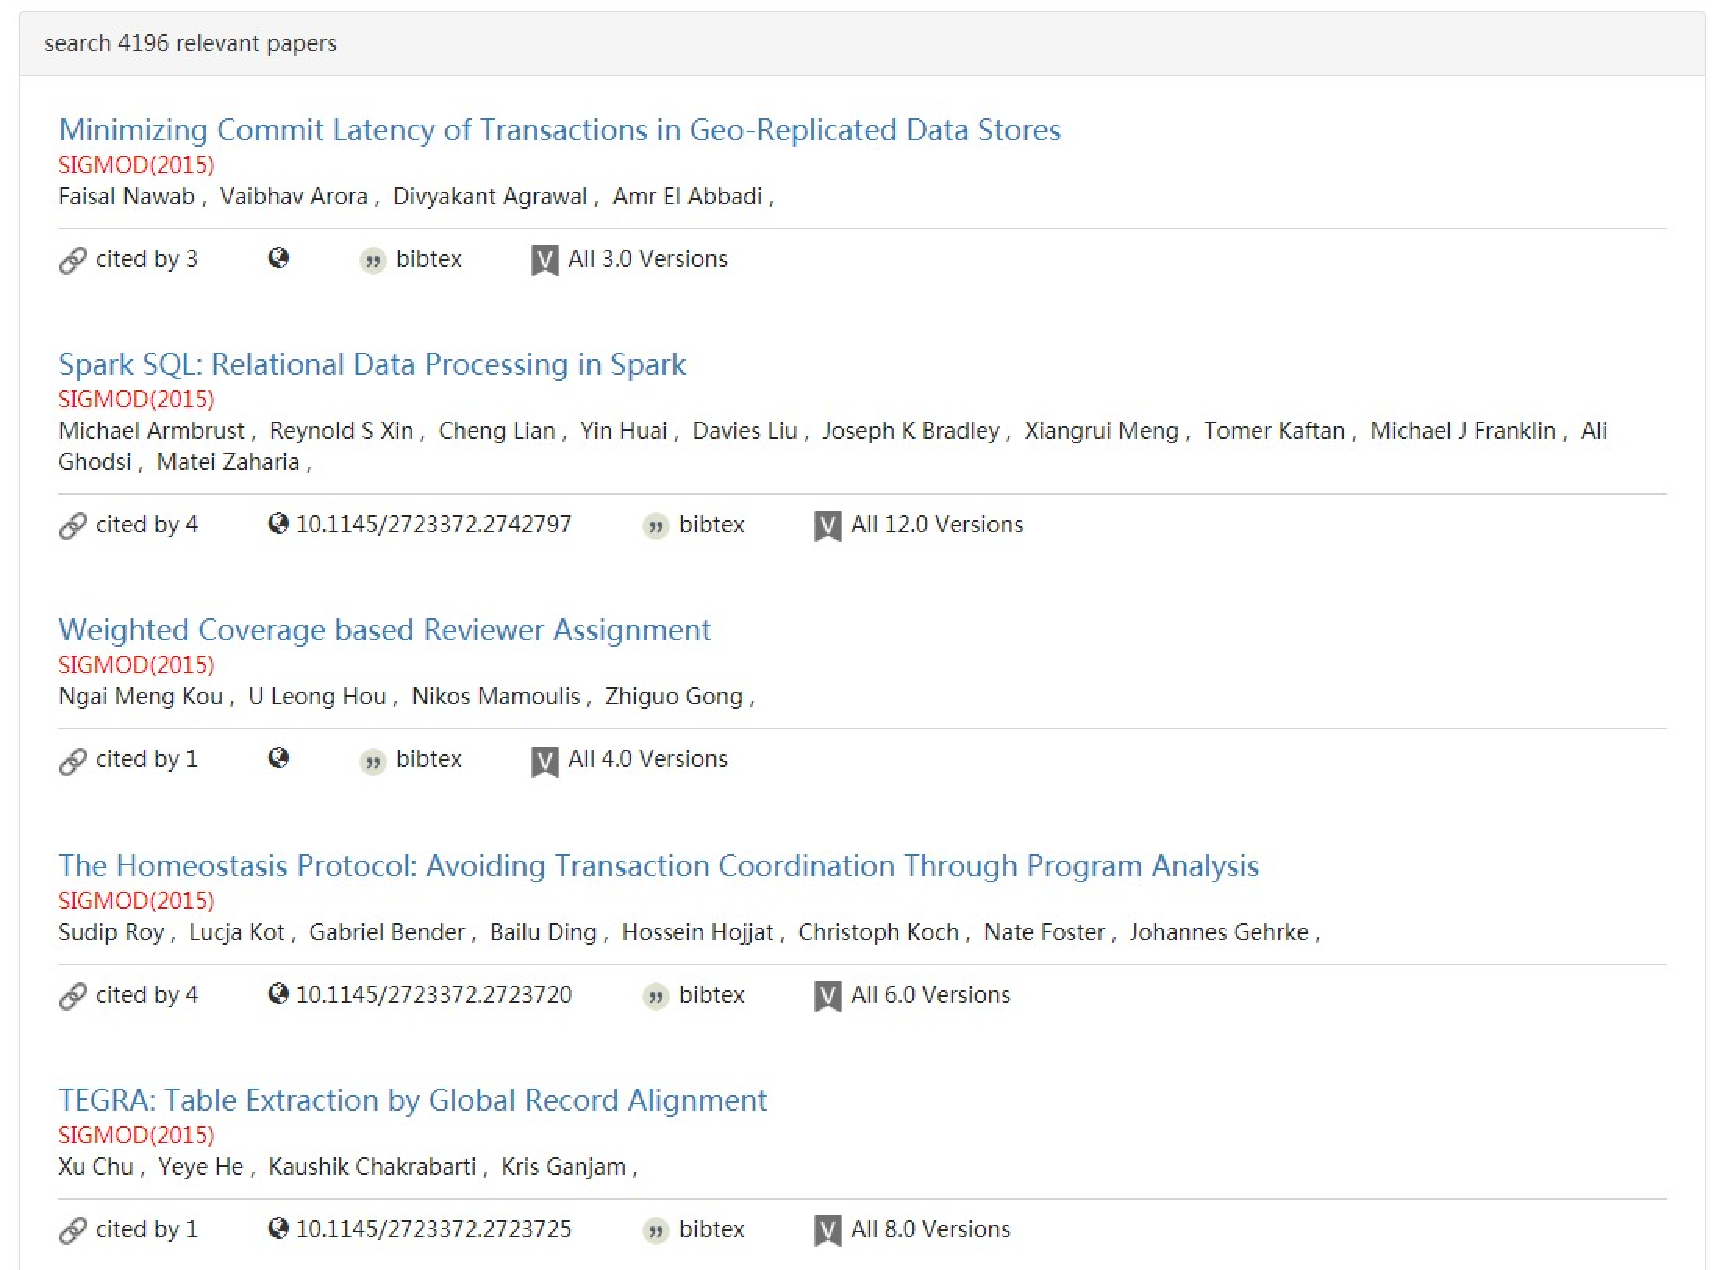
\includegraphics[width=\columnwidth]{sigmod15.pdf}
\caption{SIGMOD 2015}
\label{fig:sigmod}
\vspace{-3ex}
\end{figure}


\stitle{Author profiling}. Fig. \ref{fig:hjwProfile} is an example of an Author Page, where contains author's basic information and author's detailed profiling. For basic information, users can check author's publications, related authors and author's affiliations. We also develop author's detailed profiling to have a knowledge of the author both from breadth and depth. Thus, we model the evolution of author's research interest, author's avatar with word cloud description, the statistics of publication, {\em etc}.
%author profiling


%\par
%\stitle{Affiliation profiling}. As shown in fig. \ref{}, we give an example of affiliation profiling. The layout of the Affiliation Page is similar with Search Page, users can discover publications using various ranking metrics and check statistics information, such as the importance author, relevant affiliation, famous journals/conferences.
%% affiliation profiling

%\par
%\stitle{Venue profiling} venue
